he given set of equations can be represented in the matrix equation form as 
\begin{align}
\myvec{5&2\\3&2}\myvec{x\\y}=\myvec{3\\5}
\end{align}
The augmented matrix for this system becomes
\begin{align}
    \myvec{5&2&3\\3&2&5}
\end{align}
Row reducing the matrix
\begin{align}
   \myvec{5&2&3\\3&2&5}\xleftrightarrow[]{R_2\leftarrow R_2\times\frac{5}{3}-R_1}\myvec{5&2&3\\0&\frac{4}{3}&\frac{16}{3}}\\
    \xleftrightarrow[]{R_2\leftarrow R_2\times\frac{3}{4}}\myvec{5&2&3\\0&1&4}\\
    \xleftrightarrow[]{R_1\leftarrow R_1-2\times R_2}\myvec{5&0&-5\\0&1&4}\\
    \xleftrightarrow[]{R_1\leftarrow \frac{R_1}{5}}\myvec{1&0&-1\\0&1&4}\\
      \implies\text{Rank}\myvec{5&2\\3&2}=\text{Rank}\myvec{5&2&3\\3&2&5}=2\\=dim\myvec{5&2\\3&2}   
    \end{align}
So, the given system of equations are consistent with a unique solution of
\begin{align}
 \myvec{x\\y}=\myvec{-1\\4}   
\end{align}
\begin{figure}[!ht]
\centering
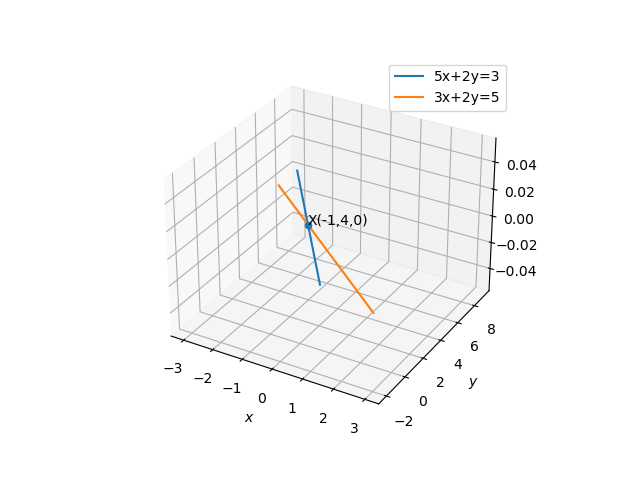
\includegraphics[width=\columnwidth]{./solutions/det/61/plot.png}
\caption{plot showing intersection of lines}
\label{Fig}
\end{figure}

